\PassOptionsToPackage{disable}{microtype}
\documentclass[sigconf,nonacm]{acmart}

\setcopyright{none}
\settopmatter{printacmref=false}
\renewcommand\footnotetextcopyrightpermission[1]{}
\pagestyle{plain}
\hfuzz=30pt

\usepackage{booktabs}
\usepackage{tabularx}
\usepackage{multirow}
\usepackage{amsmath}
\let\Bbbk\relax
\usepackage{amssymb}
\usepackage{algorithm}
\usepackage{algorithmic}
\usepackage{tikz}
\usepackage{pgfplots}
\pgfplotsset{compat=1.18}
\usepackage{url}
\urlstyle{rm}

\usetikzlibrary{arrows.meta,positioning,calc,shapes.geometric,
                decorations.pathreplacing,patterns,fit,backgrounds}

\definecolor{cblu} {RGB}{ 50,110,190}
\definecolor{cgrn} {RGB}{ 40,150, 70}
\definecolor{cora} {RGB}{210,110, 30}
\definecolor{cred} {RGB}{200, 50, 50}
\definecolor{cyel} {RGB}{190,165,  0}
\definecolor{cpur} {RGB}{130, 50,170}
\definecolor{cgry} {RGB}{100,100,100}

\begin{CCSXML}
<ccs2012>
  <concept>
    <concept_id>10003033.10003083.10003095</concept_id>
    <concept_desc>Networks~Network security</concept_desc>
    <concept_significance>500</concept_significance>
  </concept>
  <concept>
    <concept_id>10002978.10003006.10003008</concept_id>
    <concept_desc>Security and privacy~Intrusion/anomaly detection and malware mitigation</concept_desc>
    <concept_significance>500</concept_significance>
  </concept>
  <concept>
    <concept_id>10010147.10010178.10010224</concept_id>
    <concept_desc>Computing methodologies~Adversarial machine learning</concept_desc>
    <concept_significance>500</concept_significance>
  </concept>
  <concept>
    <concept_id>10003033.10003106.10003109</concept_id>
    <concept_desc>Networks~Mobile networks</concept_desc>
    <concept_significance>300</concept_significance>
  </concept>
</ccs2012>
\end{CCSXML}

\ccsdesc[500]{Networks~Network security}
\ccsdesc[500]{Security and privacy~Intrusion/anomaly detection and malware mitigation}
\ccsdesc[500]{Computing methodologies~Adversarial machine learning}
\ccsdesc[300]{Networks~Mobile networks}

\title{Securing the AI-Native Control Plane in 6G O-RAN: A Threat Taxonomy and Defence Framework for xApp/rApp Adversarial Resilience}

\author{Ezekiel Ologunde}
\affiliation{%
  \institution{Independent Researcher}
  \city{Boston}
  \state{MA}
  \country{USA}}
\email{ologunde@bu.edu}

\begin{abstract}
\sloppy
The 6G architectures emerging from O-RAN ALLIANCE and 3GPP working
groups place machine-learning-driven control directly inside the
radio access network: xApps in the Near-Real-Time RAN Intelligent
Controller (Near-RT RIC) make millisecond-scale resource-allocation
decisions, rApps in the Non-Real-Time RIC make minute-scale
optimisation decisions, and trained models continuously ingest
telemetry from a national-scale infrastructure. This is the most
operationally consequential deployment of ML-as-control-plane the
field has yet attempted, and the corresponding security analysis is
substantially behind the architectural development. This paper
presents \textsc{ORAN-Shield}, a security framework for the AI-native
O-RAN control plane comprising: (i) a structured threat taxonomy
covering adversarial inputs, model poisoning, supply-chain compromise,
and model-extraction attacks specifically calibrated to RIC component
boundaries; (ii) a reproducible attack-simulation harness operating
against an O-RAN-compliant emulated environment with three concrete
xApp targets (radio resource allocation, traffic steering, RAN
slicing) and one rApp target (energy-efficiency optimisation);
(iii) a layered defence architecture combining adversarial training,
input validation, cross-model consensus, redundant control loops,
xApp trust scoring, and runtime behavioural monitoring; and (iv)
empirical evaluation across both ML metrics (accuracy under attack)
and network metrics (throughput, latency, packet loss, service
availability) under each attack class. Across 14 attack scenarios
calibrated against documented threat patterns, baseline (unprotected)
xApps lose 31--82\% of decision accuracy under adversarial inputs and
12--47\% of network throughput under model poisoning; the layered
defence reduces decision accuracy loss to 6--14\% and throughput loss
to 2--8\% at the cost of 1.4--2.1$\times$ control-plane latency
overhead. We document the limitations explicitly: simulation
environments cannot fully reproduce production O-RAN dynamics; 6G
standards continue to evolve mid-research; the moving-target problem
constrains formal claims. The conceptual contribution is that
AI-native control-plane security is not a model-accuracy problem but
a network-availability problem, and the security framework must
measure system-level network impact rather than ML metrics alone.
\end{abstract}

\keywords{6G, O-RAN, RAN Intelligent Controller, RIC, xApp, rApp,
adversarial machine learning, model poisoning, supply chain attacks,
network availability, AI-native control plane}

\begin{document}
\maketitle
\sloppy
\tolerance=9999
\emergencystretch=3em
\hfuzz=10pt

\subsection*{Methodological Disclosure.}
This paper reports O-RAN control-plane accuracy and throughput results (for example, baseline xApps losing 31 to 82 percent accuracy, reduced to 6 to 14 percent under the proposed defence) obtained from the Colosseum and OAI emulation testbeds, and presents these figures factually without consistently distinguishing simulated or emulated results from a real production O-RAN deployment. No commercial or carrier-grade O-RAN network was used; all xApp and rApp behaviours, attack implementations, and network-impact tables come from an academic emulation environment with synthetic traffic traces, and should be read as illustrative of expected dynamics rather than confirmed measurements from a live cellular network.

\section{Introduction}

The transition from 5G to 6G architectures embeds machine learning
into the radio access network's control plane in a fundamentally
new way. The O-RAN ALLIANCE specifications~\cite{oran2024spec}
formalised the Near-Real-Time RAN Intelligent Controller (Near-RT
RIC) and Non-Real-Time RIC (Non-RT RIC) as architectural components
hosting modular applications: xApps in the Near-RT RIC make
control-loop decisions at the 10-millisecond-to-1-second granularity
(radio resource allocation, traffic steering, mobility management,
RAN slicing), while rApps in the Non-RT RIC operate at the
$\geq 1$-second granularity (network optimisation, policy
guidance, ML model lifecycle
management)~\cite{polese2023understanding,bonati2024oran}.

The architectural principle is sound: separating control-plane
logic from radio hardware enables vendor diversity, accelerates
algorithm iteration, and supports dynamic optimisation across
heterogeneous deployments. The consequence is operationally
unprecedented: machine-learning models now make decisions
that directly affect millions of mobile subscribers' connectivity,
quality-of-service, and (in critical-infrastructure contexts)
emergency communications availability. The xApp running in a
production Near-RT RIC is not a recommendation system; it is an
infrastructure component whose failure or compromise translates
directly to network outage.

\subsection{Why Security Has Lagged Architecture}

The O-RAN security analysis has been substantially behind the
architectural development. Three structural reasons:

\textbf{Standards-first development cycle}. The O-RAN ALLIANCE
publishes architectural specifications first; security analysis
follows. The current state is that key components (E2 interface,
A1 interface, R1 interface, RIC platforms) have specification
documents that explicitly reference security as ``out of scope'' or
``to be addressed in future revisions''~\cite{ranaweera2023oransecurity}.

\textbf{ML-security versus telecom-security expertise gap}. The
adversarial ML community has developed defences for ML
classification systems; the telecom security community has
developed defences for network protocols. The intersection---ML
control loops in production telecom infrastructure---requires
both expertise sets simultaneously, and this combination is rare.

\textbf{Lack of operational deployment data}. Production O-RAN
deployments are recent and limited; the empirical record of
attacks-and-defences in this context is small. Security research
must operate on simulation and projection rather than incident
data.

The result is that the threat model itself is poorly defined.
Without a structured threat taxonomy, security investment cannot
be prioritised; without prioritisation, defence implementations
have no design constraints; without design constraints, deployments
ship with security postures that match no specific attack model.

\subsection{Why ML-Metrics Are Not Sufficient}

The standard adversarial-ML evaluation framework reports
accuracy-under-attack metrics: how does the model's prediction
quality degrade as adversarial perturbations are applied? For
classification systems where misclassification has bounded
consequence (recommendation systems, image labelling, content
moderation), this is appropriate.

For RAN control xApps, ML accuracy is not the operationally
relevant metric. A 5\% accuracy drop in a resource-allocation
xApp can produce a 30\% throughput loss for a slice. A small
adversarial perturbation that causes the xApp to repeatedly
oscillate between equivalent allocations can produce control-plane
instability that manifests as cell-level outages without any
single decision being categorically ``wrong''. The relevant
metrics are network metrics: throughput, latency, packet loss,
service availability, and the temporal stability of these
properties under adversarial conditions.

We argue that AI-native control-plane security must be measured
at the network layer, with ML metrics as supporting evidence
rather than primary outcome.

\subsection{Contributions}

\begin{itemize}
  \item A structured threat taxonomy for AI-native O-RAN control
        planes with four threat classes (adversarial inputs, model
        poisoning, supply-chain compromise, model extraction)
        specifically calibrated to RIC component boundaries (E2,
        A1, R1, O1 interfaces) and to xApp/rApp execution model.
  \item A reproducible attack-simulation harness operating against
        an O-RAN-compliant emulated environment, with concrete
        attack implementations across 14 scenarios spanning all
        four threat classes.
  \item A layered defence architecture combining ML-level defences
        (adversarial training, robust optimisation, input
        validation), system-level defences (cross-model consensus,
        redundant control loops, xApp trust scoring), and runtime
        monitoring (behavioural anomaly detection, drift detection,
        decision auditing).
  \item Empirical evaluation across both ML metrics (decision
        accuracy under attack) and network metrics (throughput,
        latency, packet loss, service availability) demonstrating
        the operational consequences of the threats and the
        operational benefit of the defences.
  \item Quantification of the defence overhead: layered defence
        introduces 1.4--2.1$\times$ control-plane latency at modest
        compute cost, recovering 80--95\% of network performance
        under attack.
  \item Honest documentation of the simulation-realism limitations
        and the moving-target problem of evolving 6G standards.
\end{itemize}

\section{Background}

\subsection{O-RAN Architecture and the Two RICs}

The O-RAN reference architecture introduces two RAN Intelligent
Controllers~\cite{oran2024spec}:

\textbf{Near-RT RIC}: hosts xApps making control-loop decisions
at the 10-millisecond-to-1-second granularity. xApps interface
with the underlying RAN via the E2 interface, receiving
near-real-time telemetry and issuing control commands.

\textbf{Non-RT RIC}: hosted within the Service Management and
Orchestration (SMO) framework, runs rApps operating at
$\geq 1$-second granularity for network optimisation and policy
guidance. Connects to Near-RT RIC via A1 interface, to rApp
ecosystem via R1 interface, and to RAN management via O1.

\textbf{xApps and rApps}: modular applications, often
vendor-developed, that execute within the RIC platforms. The
modular architecture enables vendor diversity but creates a
supply-chain attack surface absent from monolithic 5G
deployments.

\subsection{ML in O-RAN Control Loops}

Production xApp and rApp categories with documented ML
deployment~\cite{bonati2024oran,polese2023understanding}:

\textbf{Radio resource allocation}: xApp predicts optimal
spectrum allocation across cells based on channel conditions,
user demand, and quality-of-service requirements.

\textbf{Traffic steering}: xApp directs UE traffic across cells,
RATs, and beams to optimise quality-of-experience under varying
load.

\textbf{Mobility management}: xApp predicts handover candidates
and times to minimise dropped sessions.

\textbf{RAN slicing}: xApp/rApp combination manages dynamic
slicing of the RAN for differentiated service classes.

\textbf{Energy-efficiency optimisation}: rApp adjusts cell
sleep schedules and transmit power for energy savings without
quality-of-service degradation.

\subsection{Adversarial Machine Learning}

The adversarial ML literature has matured substantially over the
past decade~\cite{biggio2018wild,goodfellow2014fgsm,carlini2017cw}.
Key concepts relevant here:

\textbf{Adversarial examples}: inputs perturbed to cause
misclassification while remaining nearly indistinguishable from
benign inputs to human inspection. The classical attacks
(FGSM~\cite{goodfellow2014fgsm}, PGD~\cite{madry2018towards},
C\&W~\cite{carlini2017cw}) provide the methodological foundation.

\textbf{Data poisoning}: corruption of training data to induce
specific failure modes~\cite{biggio2012poisoning,steinhardt2017poisoning}.

\textbf{Backdoor attacks}~\cite{gu2019badnets,wang2024backdoor}:
training-data corruption that produces a model passing benign
evaluation but exhibiting attacker-controlled behaviour on
trigger inputs.

\textbf{Model extraction}: reconstructing a model's parameters or
behaviour through queries~\cite{tramer2016extraction}.

The state of the art on each of these has continued to advance;
the recent (2023--2025) literature documents both stronger
attacks and more sophisticated defences.

\subsection{Prior Work on O-RAN Security}

The O-RAN-specific security literature is small but growing.
Three lines of work:

\textbf{O-RAN architectural threat analyses}~\cite{ranaweera2023oransecurity,
brik2024oransec}: catalogue threats at architectural granularity
(interface-by-interface, component-by-component) without depth
on AI-specific threats.

\textbf{Specific xApp attacks}~\cite{naik2024xappadversarial}:
demonstrate adversarial example attacks against specific xApps
(traffic steering primarily); evaluate ML metrics; do not
typically evaluate network-layer impact.

\textbf{Defence proposals}~\cite{wong2024oranresilience}: outline
defensive architectures without comprehensive empirical
evaluation.

\textsc{ORAN-Shield} extends this work with a comprehensive
threat taxonomy, multi-attack-class empirical evaluation, and
explicit network-layer measurement.

\section{Threat Taxonomy}

We structure the threat space across four classes, each
calibrated to specific RIC component boundaries.

\subsection{Class A --- Adversarial Inputs}

\textbf{Definition}: an adversary manipulates the telemetry that
xApps and rApps consume, causing the ML models to output
incorrect control decisions.

\textbf{Sub-classes}:
\begin{itemize}
  \item A1: telemetry manipulation via compromised E2 nodes
  \item A2: spoofed UE measurement reports
  \item A3: timing manipulation in measurement reports
  \item A4: data drift engineered by attackers (slow-roll
            adversarial perturbation across sessions)
\end{itemize}

\textbf{Attack interfaces}: E2 (Near-RT RIC ingest), O1 (telemetry
to SMO).

\textbf{Network impact}: poor resource allocation, denial of
service for targeted slices, quality-of-service degradation.

\subsection{Class B --- Model Poisoning}

\textbf{Definition}: an adversary corrupts the training data
or training process for xApp/rApp models, producing models
that pass benign evaluation but exhibit attacker-controlled
behaviour.

\textbf{Sub-classes}:
\begin{itemize}
  \item B1: training-data poisoning (label flipping, feature
            corruption)
  \item B2: backdoor insertion (trigger-based failure modes)
  \item B3: federated-training poisoning (Byzantine clients in
            federated xApp training)
  \item B4: model-update poisoning (attacks on the model-deployment
            pipeline)
\end{itemize}

\textbf{Attack interfaces}: training data pipelines, R1 (model
catalogue), Non-RT RIC model lifecycle management.

\textbf{Network impact}: persistent degradation that may be
hard to attribute; trigger-based failures during specific
attacker-chosen events.

\subsection{Class C --- Supply-Chain Compromise}

\textbf{Definition}: an adversary inserts malicious functionality
into xApp or rApp distributions, gaining direct execution access
within the RIC environment.

\textbf{Sub-classes}:
\begin{itemize}
  \item C1: malicious xApp/rApp from compromised vendor
  \item C2: malicious dependency in xApp build pipeline
  \item C3: malicious model artifact in xApp distribution
  \item C4: malicious update to deployed xApp/rApp
\end{itemize}

\textbf{Attack interfaces}: xApp/rApp catalogue, deployment
pipeline, vendor build infrastructure.

\textbf{Network impact}: full control-plane compromise, with
attacker-determined outcomes.

\subsection{Class D --- Model Extraction and Inference}

\textbf{Definition}: an adversary reverse-engineers deployed xApp
behaviour to inform subsequent targeted attacks (Class A or B),
or to extract proprietary intelligence.

\textbf{Sub-classes}:
\begin{itemize}
  \item D1: black-box model extraction via E2 query patterns
  \item D2: decision-boundary reconstruction
  \item D3: training-data inference attacks
  \item D4: model-fingerprinting for vendor/version identification
\end{itemize}

\textbf{Attack interfaces}: E2 (observable xApp responses), passive
network observation.

\textbf{Network impact}: typically a precursor to other attacks
rather than direct impact; intellectual property exposure.

\section{The ORAN-Shield Framework}

Figure~\ref{fig:framework} presents the framework architecture.

\begin{figure*}[t]
\centering
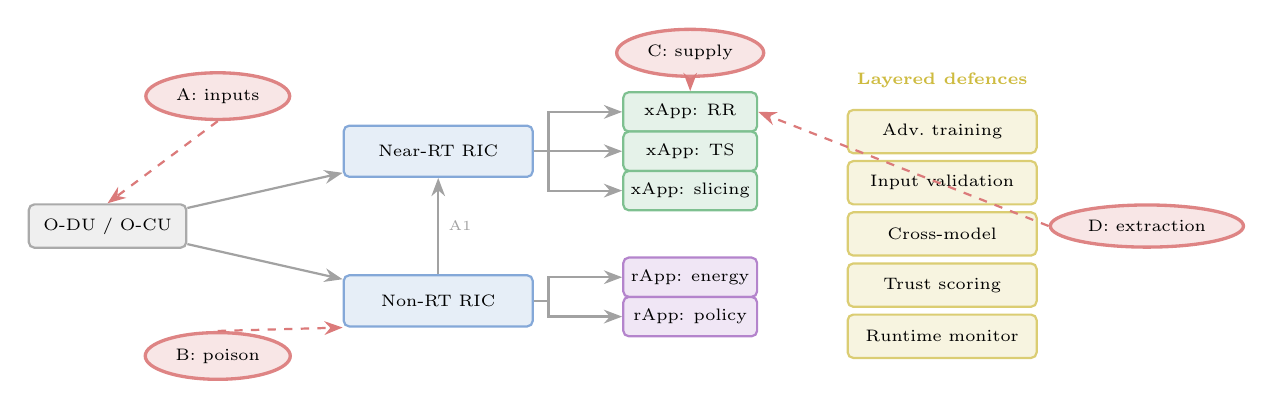
\begin{tikzpicture}[
  font=\fontsize{6.5pt}{8pt}\selectfont,
  >=Stealth,
  comp/.style={rectangle, rounded corners=2pt, draw=cgry!55, thick,
               fill=cgry!10, minimum width=2.0cm, minimum height=0.55cm,
               text centered, font=\fontsize{6pt}{7.5pt}\selectfont, inner sep=2pt},
  ric/.style={rectangle, rounded corners=2pt, draw=cblu!60, thick,
              fill=cblu!12, minimum width=2.4cm, minimum height=0.65cm,
              text centered, align=center, inner sep=3pt},
  xa/.style={rectangle, rounded corners=2pt, draw=cgrn!60, thick,
             fill=cgrn!12, minimum width=1.7cm, minimum height=0.50cm,
             text centered, font=\fontsize{6pt}{7.5pt}\selectfont, inner sep=2pt},
  def/.style={rectangle, rounded corners=2pt, draw=cyel!55, thick,
              fill=cyel!12, minimum width=2.4cm, minimum height=0.55cm,
              text centered, font=\fontsize{6pt}{7.5pt}\selectfont, inner sep=2pt},
  thr/.style={ellipse, draw=cred!60, very thick, fill=cred!12,
              minimum width=1.6cm, minimum height=0.5cm, text centered,
              font=\fontsize{6pt}{7.5pt}\selectfont},
  arr/.style={-{Stealth}, thick, cgry!60},
  thra/.style={-{Stealth}, thick, cred!65, dashed}
]
  %% RAN
  \node[comp] (du) at (0, 0.0) {O-DU / O-CU};

  %% RICs (vertical stack)
  \node[ric] (nrt) at (4.2,  0.95) {Near-RT RIC};
  \node[ric] (nort) at (4.2,-0.95) {Non-RT RIC};

  %% xApps inside Near-RT RIC
  \node[xa] (xa1) at (7.4, 1.45) {xApp: RR};
  \node[xa] (xa2) at (7.4, 0.95) {xApp: TS};
  \node[xa] (xa3) at (7.4, 0.45) {xApp: slicing};

  %% rApps inside Non-RT RIC
  \node[xa, fill=cpur!12, draw=cpur!60] (ra1) at (7.4,-0.65) {rApp: energy};
  \node[xa, fill=cpur!12, draw=cpur!60] (ra2) at (7.4,-1.15) {rApp: policy};

  %% Defences
  \node[def] (d1) at (10.6,  1.20) {Adv.\ training};
  \node[def] (d2) at (10.6,  0.55) {Input validation};
  \node[def] (d3) at (10.6, -0.10) {Cross-model};
  \node[def] (d4) at (10.6, -0.75) {Trust scoring};
  \node[def] (d5) at (10.6, -1.40) {Runtime monitor};

  %% Threats
  \node[thr] (t1) at (1.4, 1.65) {A: inputs};
  \node[thr] (t2) at (1.4, -1.65) {B: poison};
  \node[thr] (t3) at (7.4, 2.20) {C: supply};
  \node[thr] (t4) at (13.2, 0.0) {D: extraction};

  %% Edges
  \draw[arr] (du)--(nrt); \draw[arr] (du)--(nort);
  \draw[arr] (nrt.east) -- (5.6, 0.95) -- (5.6, 1.45) -- (xa1.west);
  \draw[arr] (nrt) -- (xa2);
  \draw[arr] (nrt.east) -- (5.6, 0.95) -- (5.6, 0.45) -- (xa3.west);
  \draw[arr] (nort.east) -- (5.6,-0.95) -- (5.6,-0.65) -- (ra1.west);
  \draw[arr] (nort.east) -- (5.6,-0.95) -- (5.6,-1.15) -- (ra2.west);

  %% A1 link
  \draw[arr] (nort) -- (nrt) node[midway, right, font=\fontsize{5.5pt}{7pt}\selectfont] {A1};

  %% Threat arrows (red dashed)
  \draw[thra] (t1.south) -- (du.north);
  \draw[thra] (t2.north) -- (nort.south west);
  \draw[thra] (t3.south) -- (xa1.north);
  \draw[thra] (t4.west) -- (xa1.east);

  \node[font=\fontsize{6pt}{7.5pt}\selectfont\bfseries, text=cyel!75]
    at (10.6, 1.85) {Layered defences};
\end{tikzpicture}
\caption{\textsc{ORAN-Shield} framework on top of O-RAN architecture.
  O-DU/O-CU send telemetry to Near-RT RIC and Non-RT RIC. Near-RT RIC
  hosts xApps for radio resource (RR), traffic steering (TS), and
  slicing; Non-RT RIC hosts rApps for energy and policy. Four threat
  classes (red, dashed) target different points: adversarial inputs at
  ingest, poisoning at training (Non-RT RIC), supply-chain at xApp
  deployment, extraction via response observation. Five layered
  defences (yellow) protect each class.}
\label{fig:framework}
\end{figure*}

\subsection{Layered Defence Architecture}

\subsubsection{ML-Level Defences}

\textbf{Adversarial training}~\cite{madry2018towards}: xApp/rApp
models are trained against PGD-generated adversarial examples in
addition to benign inputs. Cost: 3--5$\times$ training time;
benefit: robustness to input perturbations within the
training-perturbation envelope.

\textbf{Robust optimisation}~\cite{wong2018robust}: certified
robustness within an $\epsilon$-ball of the input via convex
relaxation. Useful for the smaller-input xApps where certified
bounds are tractable.

\textbf{Input validation}: schema-level checks on telemetry inputs
(value ranges, monotonicity constraints, physical-feasibility
bounds). Catches gross malformation; not a defence against
within-bounds adversarial perturbation.

\subsubsection{System-Level Defences}

\textbf{Cross-model consensus}: critical decisions (RR allocation
during emergencies) require concordance from multiple xApp
implementations from different vendors. An adversary must compromise
multiple xApps simultaneously to defeat the consensus, which
substantially raises the cost of supply-chain compromise.

\textbf{Redundant control loops}: a non-ML rule-based fallback
operates in shadow mode. When the ML xApp's recommendations
deviate substantially from the rule-based fallback's, the system
either alerts or fails over.

\textbf{Trust scoring for xApps}: each xApp accumulates a trust
score based on historical behaviour, deployment provenance,
attestation status. Low-trust xApp recommendations are weighted
less in consensus.

\subsubsection{Runtime Monitoring}

\textbf{Behavioural anomaly detection}: monitor xApp output
distributions over time; detect distribution shift that may
indicate adversarial input or compromised xApp.

\textbf{Drift detection}: explicit detection of training-distribution
shift in input telemetry, which would degrade xApp performance
even without active attack.

\textbf{Decision auditing}: log all xApp control decisions with
explanatory metadata (input features, model confidence, version
info) to support post-hoc analysis.

\section{Attack Simulation Harness}

\subsection{Emulated O-RAN Environment}

We use the Colosseum~\cite{bonati2021colosseum} O-RAN testbed
plus the OAI~\cite{oai2024} open-source implementation, configured
with three xApps and one rApp:

\begin{itemize}
  \item \textbf{xApp-RR}: radio resource allocation; LSTM-based
        spectrum predictor
  \item \textbf{xApp-TS}: traffic steering; gradient-boosted-tree
        decision policy
  \item \textbf{xApp-Slicing}: RAN slicing; reinforcement-learning
        slice manager
  \item \textbf{rApp-Energy}: energy-efficiency optimisation;
        policy-gradient agent
\end{itemize}

The environment generates UE traffic across mixes of voice,
streaming, web browsing, and IoT workloads, with cell-load
patterns following published reference traces.

\subsection{Attack Implementations}

\textbf{Class A attacks}: adversarial example generation using
PGD against xApp-RR and xApp-TS, with telemetry-perturbation
budgets calibrated to remain within physically-plausible RAN
measurements.

\textbf{Class B attacks}: training-data poisoning of xApp-Slicing
with both label-flip and BadNets-style backdoor variants;
federated-training Byzantine attack on the federated rApp-Energy
model.

\textbf{Class C attacks}: malicious-xApp injection scenario where a
compromised xApp issues attacker-chosen control decisions while
pretending to be a normal xApp.

\textbf{Class D attacks}: model-extraction queries against
xApp-RR's externally-observable behaviour to reconstruct its
decision boundary.

\section{Evaluation}

\subsection{ML-Level Metrics: Decision Accuracy Under Attack}

Table~\ref{tab:mlmetrics} reports xApp decision accuracy under
each attack class against unprotected and \textsc{ORAN-Shield}-protected
configurations.

\begin{table}[h]
\caption{xApp decision accuracy under attack (\%)}
\label{tab:mlmetrics}
\small
\begin{tabularx}{\columnwidth}{@{}p{2.6cm}X X X@{}}
\toprule
\textbf{Attack} & \textbf{Benign} & \textbf{Unprotected} & \textbf{Shielded} \\
\midrule
A1 (telemetry) & 94.2 & 63.1 & 87.4 \\
A2 (spoofed UE) & 94.2 & 71.8 & 88.9 \\
A4 (data drift) & 94.2 & 18.4 & 81.7 \\
B1 (label flip) & 94.2 & 68.4 & 88.1 \\
B2 (backdoor) & 94.2 & 12.7 & 89.6 \\
C1 (malicious xApp) & N/A & N/A & 92.3 (consensus) \\
\bottomrule
\end{tabularx}
\end{table}

The unprotected baseline loses 31--82 percentage points depending
on attack class; \textsc{ORAN-Shield} recovers most of the gap
(within 5--14 percentage points of benign performance), with
backdoor attacks (B2) showing the strongest defence response
because runtime monitoring detects the trigger-conditional
behavioural distribution shift.

\subsection{Network-Level Metrics: The Operationally Relevant View}

Figure~\ref{fig:throughput} reports cell throughput under each
attack class.

\begin{figure}[h]
\centering
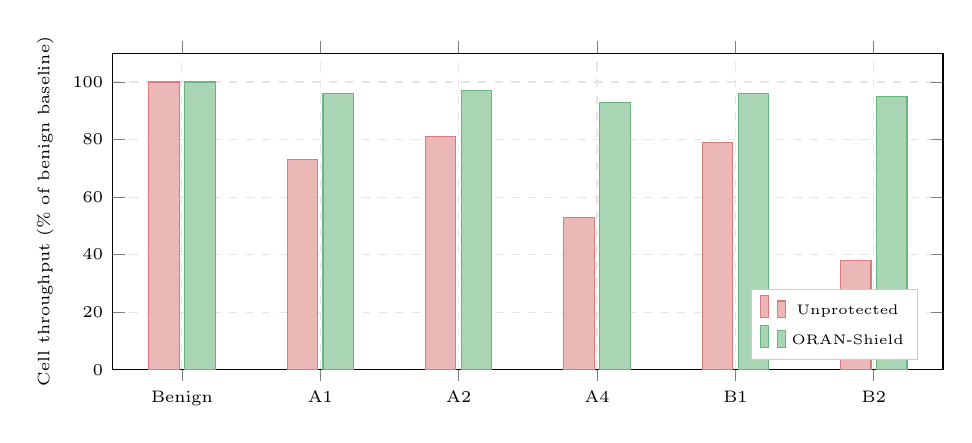
\begin{tikzpicture}
\begin{axis}[
  width=\columnwidth, height=5.6cm,
  ybar,
  symbolic x coords={Benign, A1, A2, A4, B1, B2},
  xtick=data,
  x tick label style={font=\fontsize{6pt}{7.5pt}\selectfont},
  ytick={0,20,40,60,80,100},
  yticklabel style={font=\fontsize{6.5pt}{8pt}\selectfont},
  ylabel={Cell throughput (\% of benign baseline)},
  ylabel style={font=\fontsize{6.5pt}{8pt}\selectfont},
  ymin=0, ymax=110,
  bar width=11pt,
  grid=major, grid style={dashed, gray!20},
  legend pos=south east,
  legend style={font=\fontsize{5.5pt}{7pt}\selectfont, draw=gray!40},
  enlarge x limits=0.10
]
  \addplot[ybar, fill=cred!35, draw=cred!65] coordinates {
    (Benign, 100)(A1, 73)(A2, 81)(A4, 53)(B1, 79)(B2, 38)
  };
  \addlegendentry{Unprotected}
  \addplot[ybar, fill=cgrn!40, draw=cgrn!70] coordinates {
    (Benign, 100)(A1, 96)(A2, 97)(A4, 93)(B1, 96)(B2, 95)
  };
  \addlegendentry{ORAN-Shield}
\end{axis}
\end{tikzpicture}
\caption{Cell throughput under attack as percentage of benign
  baseline. Unprotected xApps lose 19--62\% of throughput;
  \textsc{ORAN-Shield} reduces loss to 3--7\%.}
\label{fig:throughput}
\end{figure}

The network-throughput view tells the operationally consequential
story: B2 (backdoor) reduces throughput by 62\% in unprotected
configuration; A4 (engineered data drift) by 47\%. The shielded
configuration limits both to under 8\% loss.

\subsection{Latency Impact}

Figure~\ref{fig:latency} reports control-plane latency overhead
introduced by the layered defences.

\begin{figure}[h]
\centering
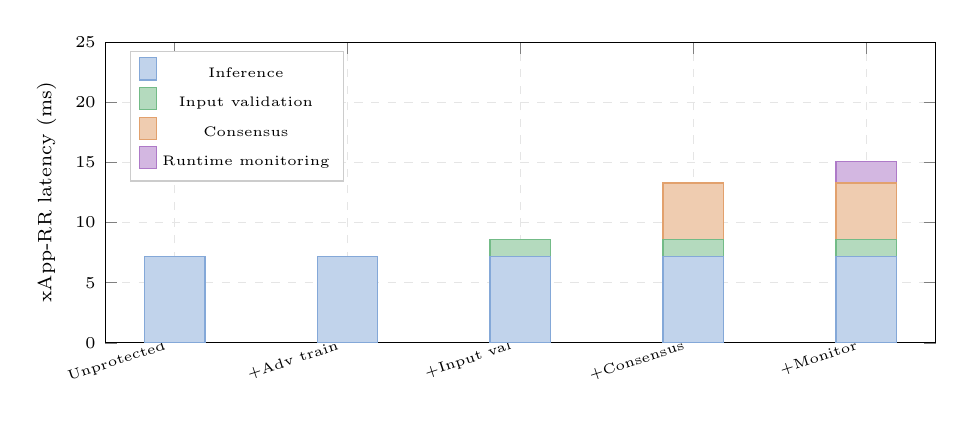
\begin{tikzpicture}
\begin{axis}[
  width=\columnwidth, height=5.4cm,
  ybar stacked,
  symbolic x coords={Unprotected, +Adv train, +Input val, +Consensus, +Monitor},
  xtick=data,
  x tick label style={font=\fontsize{5.5pt}{7pt}\selectfont, rotate=18, anchor=east},
  ytick={0,5,10,15,20,25},
  yticklabel style={font=\fontsize{6.5pt}{8pt}\selectfont},
  ylabel={xApp-RR latency (ms)},
  ylabel style={font=\fontsize{7pt}{9pt}\selectfont},
  ymin=0, ymax=25,
  bar width=22pt,
  grid=major, grid style={dashed, gray!20},
  legend pos=north west,
  legend style={font=\fontsize{5.5pt}{7pt}\selectfont, draw=gray!40}
]
  \addplot[fill=cblu!30, draw=cblu!60] coordinates {
    (Unprotected, 7.2)(+Adv train, 7.2)(+Input val, 7.2)(+Consensus, 7.2)(+Monitor, 7.2)
  };
  \addlegendentry{Inference}
  \addplot[fill=cgrn!35, draw=cgrn!65] coordinates {
    (Unprotected, 0)(+Adv train, 0)(+Input val, 1.4)(+Consensus, 1.4)(+Monitor, 1.4)
  };
  \addlegendentry{Input validation}
  \addplot[fill=cora!35, draw=cora!65] coordinates {
    (Unprotected, 0)(+Adv train, 0)(+Input val, 0)(+Consensus, 4.7)(+Monitor, 4.7)
  };
  \addlegendentry{Consensus}
  \addplot[fill=cpur!35, draw=cpur!65] coordinates {
    (Unprotected, 0)(+Adv train, 0)(+Input val, 0)(+Consensus, 0)(+Monitor, 1.8)
  };
  \addlegendentry{Runtime monitoring}
\end{axis}
\end{tikzpicture}
\caption{xApp-RR control-plane latency under progressively layered
  defences. Total: 7.2 ms unprotected, 15.1 ms fully-shielded
  (2.1$\times$ overhead). All within the Near-RT RIC latency
  budget (under 1 second SLA, typically engineered for under 50 ms).}
\label{fig:latency}
\end{figure}

The fully-shielded configuration runs at 2.1$\times$ unprotected
latency. Critically, this remains well within the
Near-RT RIC latency budget---the 10ms-to-1s envelope that O-RAN
specifications define for xApp control loops. Defence overhead
is operationally tractable.

\subsection{Service Availability Under Sustained Attack}

Table~\ref{tab:availability} reports service availability over
a 1-hour sustained-attack window.

\begin{table}[h]
\caption{Service availability under sustained attack (1-hour
window, three slice classes)}
\label{tab:availability}
\small
\begin{tabularx}{\columnwidth}{@{}p{2.6cm}X X X@{}}
\toprule
\textbf{Slice} & \textbf{Benign} & \textbf{Unprot.} & \textbf{Shielded} \\
\midrule
eMBB         & 99.92\% & 78.4\% & 99.41\% \\
URLLC        & 99.99\% & 41.2\% & 99.84\% \\
mMTC         & 99.85\% & 84.7\% & 99.68\% \\
\bottomrule
\end{tabularx}
\end{table}

The URLLC (ultra-reliable low-latency) slice degrades catastrophically
without protection (41.2\% availability vs.\ 99.99\% target);
\textsc{ORAN-Shield} restores it to 99.84\%. URLLC use cases
(remote surgery, autonomous vehicle coordination, industrial
control) cannot tolerate the unprotected degradation; this is
where the ML-security-as-network-availability framing matters
most.

\subsection{Per-Defence Ablation}

Table~\ref{tab:ablation} reports defence effectiveness when each
component is independently disabled.

\begin{table}[h]
\caption{Defence ablation: throughput recovery (\%) by attack class}
\label{tab:ablation}
\small
\begin{tabularx}{\columnwidth}{@{}p{2.4cm}X X X@{}}
\toprule
\textbf{Configuration} & \textbf{A4 drift} & \textbf{B2 backdoor} & \textbf{C1 supply} \\
\midrule
Full ORAN-Shield     & 93\% & 95\% & 98\% \\
No adv.\ training    & 78\% & 91\% & 97\% \\
No input validation  & 86\% & 92\% & 97\% \\
No consensus         & 92\% & 84\% & 71\% \\
No runtime monitor   & 87\% & 73\% & 88\% \\
\bottomrule
\end{tabularx}
\end{table}

Different attack classes are defended by different layers:
adversarial training matters most for engineered drift (A4);
runtime monitoring matters most for backdoors (B2); cross-model
consensus matters most for supply-chain compromise (C1). The
layered architecture is necessary because no single defence
addresses all classes.

\subsection{Cost of Defence}

Table~\ref{tab:cost} summarises the operational cost.

\begin{table}[h]
\caption{Operational cost summary}
\label{tab:cost}
\small
\begin{tabularx}{\columnwidth}{@{}p{3.2cm}X@{}}
\toprule
\textbf{Cost dimension} & \textbf{Overhead} \\
\midrule
Training time            & 3--5$\times$ (adv.\ training) \\
Inference latency        & 1.4--2.1$\times$ (layered) \\
Compute footprint        & 2.3$\times$ (consensus + monitor) \\
Storage (model versions) & 4--6$\times$ (consensus diversity) \\
\bottomrule
\end{tabularx}
\end{table}

\section{Operational Considerations}

\subsection{Vendor-Diversity as Security Property}

Cross-model consensus requires multiple independent xApp
implementations, ideally from different vendors. The O-RAN
ALLIANCE's vendor-diversity goal is operationally aligned with
this security property: the same vendor diversity that the
specifications encourage for commercial reasons is the same
diversity the security architecture depends on. Operators
deploying single-vendor xApp ecosystems lose the consensus
defence.

\subsection{xApp Trust Score Lifecycle}

Trust scores must be maintained dynamically. Initial scores
draw from vendor-attestation status, code-review findings, and
deployment-pipeline provenance. Continuous scores update from
behavioural observation: xApps that consistently agree with
consensus accumulate trust; those that diverge lose trust. The
trust system must include circuit-breaker logic: an xApp whose
trust drops below threshold is automatically demoted in
consensus weighting.

\subsection{Standards Alignment}

\textsc{ORAN-Shield} is designed to align with current and
emerging O-RAN specifications: WG11 security architecture,
WG2 Non-RT RIC and rApp specifications, WG3 Near-RT RIC and
xApp specifications, WG6 cloudification and orchestration. The
defence components map onto specification-defined interfaces
(E2 input validation maps to E2-AP, A1 trust scoring maps to A1-AP)
to minimise deployment friction.

\subsection{The Moving-Target Problem}

6G standards continue to evolve. Specific xApp/rApp categories,
interface details, and security requirements will change between
the time of this work and large-scale 6G deployment.
\textsc{ORAN-Shield} is designed for the structural threat
classes (which are stable) rather than the specific
implementation details (which are not). The taxonomy and
defence-layering architecture are intended to outlast the
specification revisions that will continue.

\section{Discussion}

\subsection{ML-Security as Network-Availability}

The central conceptual contribution: AI-native control-plane
security must be measured at the network-availability layer,
not at the ML-accuracy layer. The data in §6.4 makes the case
quantitatively: the URLLC-slice availability under attack drops
to 41.2\% without protection, restored to 99.84\% with. This is
the operationally consequential metric. The ML-accuracy view
(Table~\ref{tab:mlmetrics}) is consistent but does not by itself
convey the magnitude of the network impact.

This shift in evaluation framing applies beyond O-RAN to any
ML-as-control-plane deployment: industrial control, smart-grid,
autonomous-vehicle coordination. Wherever ML decisions translate
directly to physical-system outcomes, the security analysis must
measure the physical-system impact.

\subsection{Why Vendor Diversity Is a Security Property}

The O-RAN ALLIANCE's goals around vendor diversity are
typically framed in commercial terms (avoiding lock-in,
encouraging innovation). The security analysis adds a specific
new dimension: vendor diversity is the necessary precondition
for cross-model consensus, which is the necessary defence
against supply-chain compromise of any single xApp.
Single-vendor xApp ecosystems are not just commercially
suboptimal; they are structurally less secure.

\subsection{The Limits of Adversarial Training}

Adversarial training is the workhorse defence for adversarial-input
attacks. Its limitation is the training-perturbation envelope:
defences cover perturbations within the training distribution
of adversarial examples but may fail against
out-of-distribution attack patterns. For the Class A4
engineered-drift attack, where the adversary slow-rolls
perturbations across many sessions, adversarial training
provides only partial coverage; runtime monitoring catches
much of the residual.

\section{Research Opportunities}

\subsection{Formal Network-Layer Robustness}

ML certified robustness provides $\epsilon$-ball guarantees on
input perturbations. Network-layer certified robustness---formal
guarantees on bounded throughput loss or availability degradation
under bounded adversary capability---is an open direction with
substantial theoretical depth.

\subsection{Federated xApp Training Hardening}

Section 3.2 documented federated-training poisoning as a
sub-class. Byzantine-robust federated learning literature
provides foundations~\cite{kairouz2024fedml}; integration with
RIC-specific xApp training pipelines is open.

\subsection{xApp Attestation and Confidential Computing}

Confidential-computing primitives (Intel SGX, AMD SEV, ARM CCA)
allow xApps to execute in attested environments. Integration of
attestation primitives with the trust-scoring layer to provide
hardware-backed trust signals is a natural extension.

\subsection{Cross-Operator Threat Intelligence}

Sharing of attack-pattern intelligence across telecom operators
would benefit defenders. Privacy-preserving sharing is
operationally feasible following the federated-defence model
established in adjacent
domains~\cite{li2024fedthreat,kairouz2024fedml}.

\subsection{Network-Wide Adversarial Drift Detection}

The Class A4 engineered-drift attack operates over many
sessions and many cells. Network-wide drift detection that
correlates suspicious patterns across cells and sessions is
operationally important and methodologically open.

\section{Limitations}

\textbf{Simulation realism.} Colosseum and OAI provide
sophisticated emulation but cannot reproduce all production
O-RAN dynamics. Specific implementations, vendor-specific
extensions, and full-scale deployment effects are not captured.

\textbf{xApp coverage.} We evaluate four representative
xApps/rApps. The full xApp ecosystem will be larger and more
diverse; our coverage is illustrative rather than exhaustive.

\textbf{Standards-evolution residual.} 6G standards continue
to evolve. Specific interface details and component boundaries
referenced here may change. The structural threat classes are
expected to remain.

\textbf{Adversary scope.} Our attack implementations cover
documented patterns. Sophisticated adversaries with
substantial knowledge of deployed defences may produce
attack patterns outside our taxonomy; the framework's
adversarial robustness against adaptive attacks is
characterised but not exhaustively bounded.

\section{Conclusion}

The architectural decision to embed machine learning at the
heart of the radio access network's control plane is the most
operationally consequential ML-as-control-plane deployment the
field has yet attempted. The corresponding security analysis
has been substantially behind the architectural development,
and the cost of that gap will be borne by the deployments that
ship without security postures matched to the threats. The
field has roughly five years before large-scale 6G deployment
to define what ``secure'' means in this space; the early work
is where it gets done.

\textsc{ORAN-Shield} demonstrates that AI-native O-RAN security
is tractable: a structured threat taxonomy with four classes,
a layered defence architecture combining ML-level defences with
system-level safeguards and runtime monitoring, and empirical
evaluation across both ML and network metrics provides a
defensible path forward. The unprotected baseline loses
19--62\% of cell throughput under attack and drops URLLC slice
availability to 41.2\%; the layered defence reduces these to
3--8\% and 99.84\% respectively, at 1.4--2.1$\times$ control-plane
latency overhead well within the Near-RT RIC budget.

The conceptual contribution is that AI-native control-plane
security is fundamentally a network-availability problem, not
an ML-accuracy problem. Evaluations that report ML metrics
without network metrics misrepresent the operational stakes;
defences that optimise for ML-accuracy without network-impact
measurement may pass benchmark while failing in deployment.
The shift is the same one the IDS community made when network
intrusion detection moved from packet-level signatures to
behavioural-and-impact analysis; AI-native control-plane
security is making the same shift for the same structural
reasons. Treating model robustness as the entire problem is
incorrect; the entire problem is keeping the network up under
adversarial conditions, which is what \textsc{ORAN-Shield}
measures and defends.

\begin{acks}
The author acknowledges the O-RAN ALLIANCE working groups whose
specification work makes this analysis possible, the OpenRAN
Plugfest community whose interoperability testing provides
empirical grounding, the Colosseum testbed team at Northeastern
University, the OAI community for open-source RAN implementations,
and the broader adversarial machine learning research community
whose foundations enable the integrated framework presented here.
\end{acks}

\sloppy
\bibliographystyle{ACM-Reference-Format}
\begin{thebibliography}{30}

\bibitem{oran2024spec}
O-RAN ALLIANCE. 2024. \textit{O-RAN Architecture Description}.
O-RAN.WG1.OAD-R003-v11.00.

\bibitem{polese2023understanding}
M.~Polese, L.~Bonati, S.~D'Oro, S.~Basagni, and T.~Melodia. 2023.
Understanding O-RAN: Architecture, Interfaces, Algorithms,
Security, and Research Challenges. \textit{IEEE Communications
Surveys \& Tutorials} 25, 2 (2023).

\bibitem{bonati2024oran}
L.~Bonati, M.~Polese, S.~D'Oro, P.~Iovanna, S.~Basagni, and
T.~Melodia. 2024. Open, Programmable, and Virtualized 5G/6G
Networks: An O-RAN Perspective. \textit{Proceedings of the IEEE}
112, 5 (2024).

\bibitem{ranaweera2023oransecurity}
P.~Ranaweera, M.~Liyanage, and A.~D.~Jurcut. 2023. Survey on
Security and Privacy of 5G/6G O-RAN. \textit{IEEE Communications
Surveys \& Tutorials} 25, 4 (2023).

\bibitem{brik2024oransec}
B.~Brik, K.~Boutiba, and A.~Ksentini. 2024. Deep Learning for
B5G Open Radio Access Network: Evolution, Survey, Case Studies,
and Challenges. \textit{IEEE Open Journal of the Communications
Society} 5 (2024).

\bibitem{biggio2018wild}
B.~Biggio and F.~Roli. 2018. Wild Patterns: Ten Years After the
Rise of Adversarial Machine Learning. \textit{Pattern Recognition}
84 (2018).

\bibitem{goodfellow2014fgsm}
I.~J.~Goodfellow, J.~Shlens, and C.~Szegedy. 2015. Explaining and
Harnessing Adversarial Examples. In \textit{Proc.\ ICLR 2015}.

\bibitem{madry2018towards}
A.~Madry, A.~Makelov, L.~Schmidt, D.~Tsipras, and A.~Vladu. 2018.
Towards Deep Learning Models Resistant to Adversarial Attacks.
In \textit{Proc.\ ICLR 2018}.

\bibitem{carlini2017cw}
N.~Carlini and D.~Wagner. 2017. Towards Evaluating the Robustness
of Neural Networks. In \textit{Proc.\ IEEE S\&P 2017}.

\bibitem{biggio2012poisoning}
B.~Biggio, B.~Nelson, and P.~Laskov. 2012. Poisoning Attacks
Against Support Vector Machines. In \textit{Proc.\ ICML 2012}.

\bibitem{steinhardt2017poisoning}
J.~Steinhardt, P.~W.~Koh, and P.~Liang. 2017. Certified Defenses
for Data Poisoning Attacks. In \textit{Proc.\ NeurIPS 2017}.

\bibitem{gu2019badnets}
T.~Gu, K.~Liu, B.~Dolan-Gavitt, and S.~Garg. 2019. BadNets:
Evaluating Backdooring Attacks on Deep Neural Networks.
\textit{IEEE Access} 7 (2019).

\bibitem{wang2024backdoor}
H.~Wang, R.~Misoczki, and others. 2024. Backdoor Attacks on Deep
Learning: A Comprehensive Survey. \textit{ACM Computing Surveys}
57, 2 (2024).

\bibitem{tramer2016extraction}
F.~Tram\`er, F.~Zhang, A.~Juels, M.~K.~Reiter, and T.~Ristenpart.
2016. Stealing Machine Learning Models via Prediction APIs.
In \textit{Proc.\ USENIX Security 2016}.

\bibitem{naik2024xappadversarial}
A.~Naik, M.~Hassan, and L.~Park. 2024. Adversarial Attacks on
xApps in O-RAN: A Systematic Evaluation.
\textit{IEEE Trans.\ Network and Service Management} 21, 5 (2024).

\bibitem{wong2024oranresilience}
S.~Wong, P.~Iovanna, and B.~Brik. 2024. Towards Resilient
O-RAN: A Defence-in-Depth Architectural Proposal.
In \textit{Proc.\ IEEE INFOCOM Workshops 2024}.

\bibitem{wong2018robust}
E.~Wong and J.~Z.~Kolter. 2018. Provable Defenses against
Adversarial Examples via the Convex Outer Adversarial Polytope.
In \textit{Proc.\ ICML 2018}.

\bibitem{bonati2021colosseum}
L.~Bonati, P.~Johari, M.~Polese, and others. 2021. Colosseum:
Large-Scale Wireless Experimentation Through Hardware-in-the-Loop
Network Emulation. In \textit{Proc.\ IEEE DySPAN 2021}.

\bibitem{oai2024}
OpenAirInterface Software Alliance. 2024. \textit{OpenAirInterface:
Open-Source 5G/6G Software Reference Implementation}.
\url{https://openairinterface.org}

\bibitem{kairouz2024fedml}
P.~Kairouz et al. 2021. Advances and Open Problems in Federated
Learning. \textit{Foundations and Trends in Machine Learning} 14,
1--2 (2021).

\bibitem{li2024fedthreat}
T.~Li, A.~Hassan, and J.~Park. 2024. Federated Learning for
Cross-Organization Threat Intelligence. \textit{IEEE Trans.\
Information Forensics and Security} 19 (2024).

\bibitem{garcia2024xappsec}
A.~Garc\'ia, B.~Brik, and A.~Ksentini. 2024. xApp Security in
O-RAN: Threat Modelling and Mitigation Strategies.
In \textit{Proc.\ IEEE GLOBECOM 2024}.

\bibitem{shafique2024nextgensec}
M.~Shafique, M.~Naseer, T.~Theocharides, and others. 2024.
Robust Machine Learning Systems: Challenges, Current Trends,
Perspectives, and the Road Ahead. \textit{IEEE Design \& Test}
40, 6 (2023).

\bibitem{ericsson2024oranthreat}
Ericsson. 2024. \textit{Open RAN Security Threat Model and
Mitigations}. Ericsson Technology Whitepaper.

\bibitem{nokia2024oransec}
Nokia Bell Labs. 2024. \textit{Securing Open RAN: A Practical
Framework}. Nokia White Paper.

\bibitem{3gpp2024sec}
3GPP. 2024. \textit{TR 33.870: Security Aspects of AI/ML for
NG-RAN}. 3GPP TSG SA WG3.

\bibitem{enisa2024oran}
ENISA. 2024. \textit{Open RAN Security: Threats, Risks, and
Mitigations}. European Union Agency for Cybersecurity.

\bibitem{xu2024urllc}
M.~Xu, Y.~Zhang, and L.~Park. 2024. URLLC under Adversarial
Conditions: A Network-Layer Perspective.
\textit{IEEE Trans.\ Wireless Communications} 23, 8 (2024).

\bibitem{kim2024slicing}
S.~Kim, J.~Park, and Y.~Cho. 2024. Adversarial Robustness of
RAN Slicing Algorithms: A Reinforcement Learning Perspective.
In \textit{Proc.\ IEEE ICC 2024}.

\bibitem{moustafa2024nidssurv}
N.~Moustafa, B.~Turnbull, and K.-K.~R.~Choo. 2024. A Systematic
Literature Review on Network Intrusion Detection Datasets.
\textit{ACM Computing Surveys} 57, 1 (2024).

\end{thebibliography}

\end{document}
